%TODO: add intro to the sections
\section{Mobile technology}

After the introduction of smartphones, there has been an explosive surge in the
popularity of using mobile technologies as computers.
\begin{figure}[!ht]
\centering
\subfigure{
  
\includegraphics[scale=0.06]{pictures/android}
}
\subfigure{
  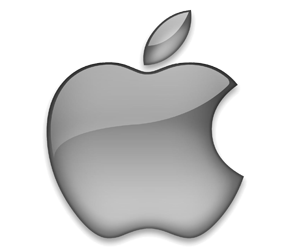
\includegraphics[scale=0.2]{pictures/apple-logo}
}
\subfigure{
  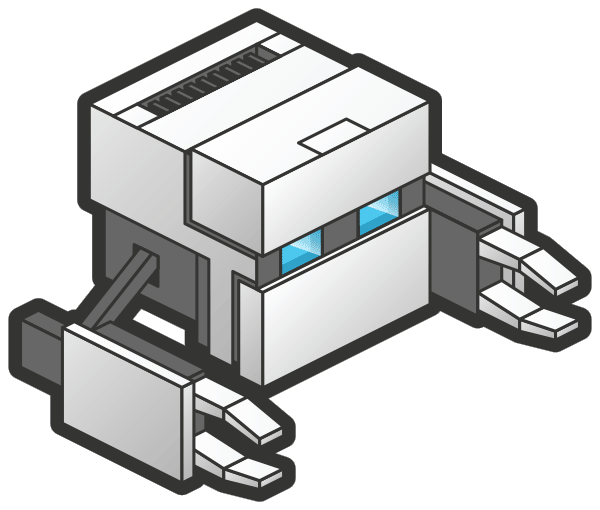
\includegraphics[scale=0.1]{pictures/phonegap}
}
\subfigure{
  
\includegraphics[scale=0.13]{pictures/css3}
}
\linebreak
\subfigure{
  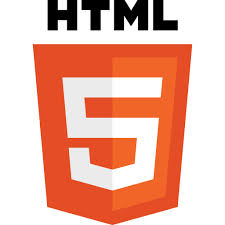
\includegraphics[scale=0.245]{pictures/html5}
}
\subfigure{
  
\includegraphics[scale=0.12]{pictures/corona}
}
\subfigure{
  
\includegraphics[scale=0.25]{pictures/js}
}
\caption{Android, IOS, Phonegap, CSS3, HTML5, Corona and Javasript}
\end{figure}

\subsection{Mobile platforms}
{\bf Android} is a Linux-based operating system, designed primarily for mobile
devices with touch screen support. Android is currently being developed by
Google and is deployed on various mobile devices developed by third parties.
Source: \url{http://en.wikipedia.org/wiki/Android_(operating_system)}
\linebreak

\indent
  {\bf Pros:}
  \begin{itemize}
    \item Developing for Android is free.
    \item Native support for Java, a well known programming language.
    \item Android apps can be developed on any of the major desktop operating
          systems.
    \item Android can be emulated using an AVD (Android Virtual Device),
          allowing for easy testing.
  \end{itemize}

\indent
  {\bf Cons:}
  \begin{itemize}
    \item There are many different Android devices, making testing more
          demanding.
    \item Apps developed for Android will only run on Android.
  \end{itemize}

\noindent
{\bf iOS} is an operating system developed by Apple primarily for the iPhone,
which has been extended to run on other Apple devices such as the iPad. Apple
does not allow iOS to be deployed on non-Apple hardware.
Source: \url{http://en.wikipedia.org/wiki/IOS}

\indent
  {\bf Pros:}
  \begin{itemize}
    \item There are fewer devices running iOS, and things like screen
          resolution is typically standardized, making development and testing
          easier.
  \end{itemize}

\indent
  {\bf Cons:}
  \begin{itemize}
    \item Apple hardware and software required to develop for iOS.
    \item Distribution of applications for iOS requires a yearly subscription.
    \item Apple's App Store enforces strict terms of distribution which may not
          be compatible with other software licences.
    \item Apps developed for iOS will only run on iOS.
  \end{itemize}


\subsection{Cross-platform}
    {\bf PhoneGap} is a free and open source framework that makes it possible
    to create mobile applications using web technologies like HTML, CSS and
    JavaScript. PhoneGap allows developers to create an application which is a
    hybrid between a web app and a native application. PhoneGap packages the
    program as an application and gives the developer access to native device APIs.
    Source: \url{http://phonegap.com/about/}

\indent
  {\bf Pros:}
  \begin{itemize}
    \item Applications can be developed for Android, BlackBerry, iOS,
          Windows Phone, Windows 8 and Tizen operating systems.
    \item PhoneGap apps are developed using well known technologies such as
          JavaScript, HTML and CSS.
    \item Access to native APIs like camera, storage, networking,
          touch screen etc.
    \item Existing CSS and JavaScript libraries can be leveraged.
    \item Looks like a native application.
    \item Makes it easy to build applications for all supported platforms.
    \item PhoneGap is open source.
  \end{itemize}

\indent
{\bf Cons:}
  \begin{itemize}
    \item PhoneGap runs as an offline webpage, which is likely to impact
          performance.
  \end{itemize}

\noindent
{\bf Corona} is a software development kit (SDK) which allows developers to
build applications for iPhone, iPad and Android devices. Corona is not open
source, and enforces a revenue limit for developers unless the developers pay a
monthly fee. Corona lets programmers develop using Lua.
Source: \url{http://www.coronalabs.com/products/corona-sdk/}

\indent
  {\bf Pros:}
  \begin{itemize}
    \item Comes with a physics engine and other features useful for game
          development.
  \end{itemize}

\indent
  {\bf Cons:}
  \begin{itemize}
    \item Not open source
    \item Costs money to unlock full feature set.
  \end{itemize}

\subsection{Native}
For focus on single platforms, developing native applications would probably be
the best choice. Native applications for Android are developed using the Java
programming language whereas iOS apps are developed in Objective-C.

\indent
  {\bf Pros:}
  \begin{itemize}
    \item Easier to ensure that the application will run on all versions of
          the platforms.
    \item Best performance.
  \end{itemize}

\indent
  {\bf Cons:}
  \begin{itemize}
    \item We have to develop for both iOS and Android in different languages.
          Both of these apps would have to be maintained in parallel.
    \item We will have to learn Objective-C.
    \item Can only build applications for iOS on Mac.
  \end{itemize}

\noindent
\subsection{Conclusions}
    After having discussed it in the group and with the customer we have agreed
    on using PhoneGap to develop the game. The customer wanted the game to
    be developed with known technology that they can easily find people with
    experience with. HTML, CSS and JavaScript constitute a very popular development
    platform.
